\begin{artplenv2auth}{Marcin Miłkowski, Witold Wachowski}
	{Hutchins w~obronie interdyscyplinarnych badań nad poznaniem}
	{Hutchins w~obronie interdyscyplinarnych badań nad poznaniem}
	{Hutchins w~obronie interdyscyplinarnych badań nad poznaniem}
	{\flushright\subbold{Marcin Miłkowski}\\\subsubsectit\small{Polish Academy of Sciences}\par
		\flushright\subbold{Witold Wachowski}\\\subsubsectit\small{Maria Curie-Skłodowska University}\par}
	{Edwin Hutchins: In defense of interdisciplinary research on cognition}
	{The article presents the interdisciplinary approach of Edwin Hutchins, analyzing his conception of distributed cognition as probably the most important and lasting contribution of anthropology to the repertoire of theoretical tools in cognitive science. At the same time, this conception resulted in one of the most interesting relationships between cognitive science and social sciences. These relationships are made possible by the assumptions of Hutchins' conception, which directly contribute to interdisciplinary collaboration. His account of distributed cognition has enormous potential, allowing the integration of research into cognitive and social processes. This is also because it breaks with methodological individualism.}
	{cognitive anthropology, ethnography, methodological individualism, cognitive science, distributed cognition, representational states, interdisciplinarity.}
		{\flushright\subbold{Marcin Miłkowski}\\\subsubsectit\small{Polish Academy of Sciences}\par
			\flushright\subbold{Witold Wachowski}\\\subsubsectit\small{Maria Curie-Skłodowska University}\par}
	
	


\section{Wprowadzenie}
\lettrine[loversize=0.13,lines=2,lraise=-0.01,nindent=0em,findent=0.2pt]%
{A}{}ntropologia jako jeden z~głównych filarów kognitywistyki podejmuje zagadnienia nauk poznawczych i~społecznych. Jeżeli więc szukać zależności i~oddziaływań między nimi, nie sposób tej dziedziny nie uwzględnić: wydaje się, że to głównie ona powinna łączyć kognitywistykę (czyli interdyscyplinarny konglomerat badań nad poznaniem) z~prowadzonymi przez antropologów poznawczych czy socjologów wiedzy badaniami nad społecznymi procesami poznawczymi. A~jednak historia decydującego udziału antropologii w~kognitywistyce jest stosunkowo krótka. Wydaje się, że pozostał po niej jeden wyróżniający się i~rozwijany po dziś dzień nurt, mianowicie badania nad poznaniem rozproszonym; ich najbardziej zasłużonym i~rozpoznawanym przedstawicielem jest Edwin Hutchins
%\label{ref:RNDTItwQrjVZ5}(2022).
\parencite*[][]{hutchins_hutchins_2022}.%




Przyjrzyjmy się jednak historycznym perturbacjom poprzedzającym te badania. Wymowną pamiątką po początkowym równorzędnym udziale antropologii w~powstawaniu kognitywistyki jest klasyczny heksagram z~1978 roku
%\label{ref:RNDSBQnKnGe0V}(zob. np. Miller, 2003),
\parencite[zob. np. ][]{miller_cognitive_2003}, %
 obrazujący udział sześciu dyscyplin: językoznawstwa, neurobiologii, sztucznej inteligencji, filozofii, psychologii oraz właśnie antropologii (patrz Ilustracja \ref{fig1milk}). Wydaje się, że kognitywiści tamtych czasów doceniali społeczno-\mbox{-kulturowe} aspekty procesów poznawczych, toteż antropologia pozostawała w~tamtym czasie w~dość dobrych relacjach z~kognitywistyką 
%\label{ref:RNDEcfkRYeL7r}(Bender, i~in., 2010).
\parencite[][]{bender_anthropology_2010}. %
 Allen Newell 
%\label{ref:RNDNDK3R4x7hN}(Newell, 1980, 1990)
\parencites*[][]{newell_physical_1980}[][]{newell_unified_1990} %
 wymieniał społeczne aspekty poznania wśród swoich 13 kryteriów ujednoliconej teorii poznawczej. Donald Norman 
%\label{ref:RND9s1QItJbxy}(1981),
\parencite*[][]{norman_twelve_1981}, %
 będący jednocześnie klasykiem badań nad poznaniem oraz przedstawicielem koncepcji poznania rozproszonego, wskazywał na systemy wiedzy kulturowej wśród 12 kluczowych zagadnień w~kognitywistyce. Z~kolei Howard Gardner 
%\label{ref:RNDGYeAGaHSe1}(1985)
\parencite*[][]{gardner_minds_1985} %
 wymieniał emocje, kontekst, kulturę i~historię jako istotne elementy aktywności poznawczej. W~ten sposób udział antropologii otwierał przed kognitywistyką perspektywę systematycznych dociekań nad kulturowymi mechanizmami systemów wiedzy, z~uwzględnieniem ograniczeń poznawczych i~ekologicznych.
 

\begin{figure}
\begin{center}
 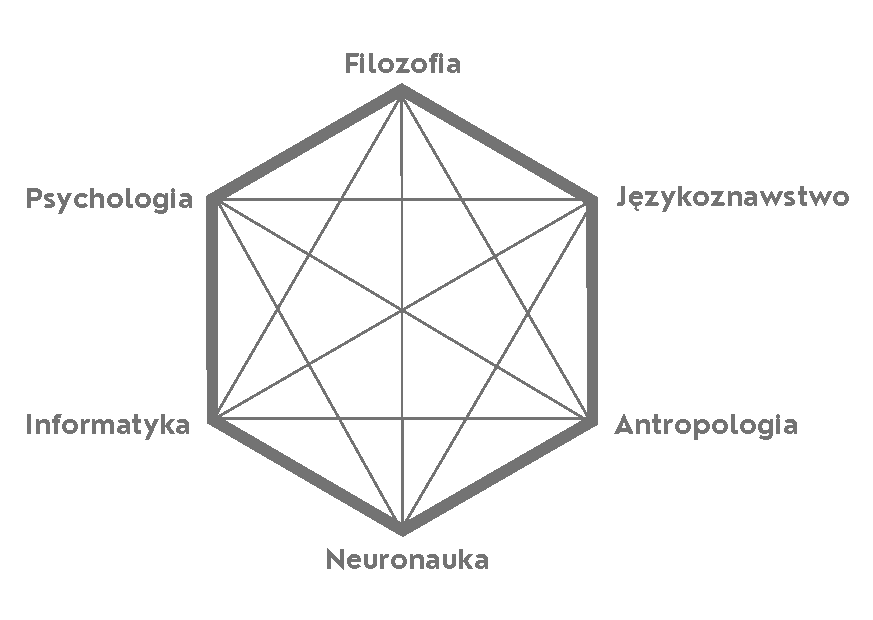
\includegraphics[width=.9\textwidth]{ART_milkowski/ilustracja1pu.pdf}
\end{center}
 \caption{Heksagram obrazujący udział sześciu dyscyplin: językoznawstwa, neurobiologii, sztucznej inteligencji, filozofii, psychologii oraz antropologii w powstawaniu kognitywistyki.}\label{fig1milk}
\end{figure}

Co się jednak stało, że ostatecznie wykluczono rolę społeczeństwa i~kultury z~głównego nurtu kognitywistyki, doprowadzając przy tym do rozejścia się dróg antropologów i~kognitywistów? Za jedną z~przyczyn uważa się rozłam w~samej antropologii na obszar przyrodniczo-\mbox{-ścisły} i~humanistyczny, gdzie antropologia poznawcza, wykazująca cechy obu, okazała się ,,niekochanym dzieckiem'', którym nie zaopiekowało się żadne z~,,rodziców''. Również sama współpraca antropologów z~kognitywistami pozostawiała sporo do życzenia. Tych pierwszych zniechęcały preferowane przez drugich ściśle kontrolowane eksperymenty, prowadzone w~sztucznych warunkach laboratoryjnych, przy niedocenianiu roli kontekstu i~realnych warunków. Kognitywiści z~kolei zarzucali antropologom brak odpowiedniego rygoru badawczego i~nadmierne skupienie na danych jakościowych. James Boster podkreślał, że antropologia, w~odróżnieniu od psychologii w~kognitywistyce, ,,skupia się na treści (nie na procesie), na społecznościach i~kontekstach społecznych (nie na jednostkach), na warunkach naturalnych (nie laboratoryjnych), na uchwytywaniu zjawisk w~świecie rzeczywistym, nawet jeśli wymaga to pewnego złagodzenia rygorów, i~troszczy się o~to, czy zebrane dane faktycznie dowodzą tego, co może się wydawać na pierwszy rzut oka''
%\label{ref:RNDyjHJO3J9ub}(za Bender, i~in., 2010, s.~377; przekład własny).
\parencite[za ][s.~377; przekład własny]{bender_anthropology_2010}. %
 Dodajmy, że do podtrzymania tego stanu rzeczy przyczynili się również kontynuatorzy Newella, eliminując rolę społeczeństwa i~kultury z~projektu formowania jednolitej teorii poznania 
%\label{ref:RNDIkQobHmtSa}(Hutchins, 1995a; Bender, i~in., 2010; Anderson, Lebiere, 2003; Kronenfeld, i~in., 2011).
\parencites[][]{hutchins_cognition_1995}[][]{bender_anthropology_2010}[][]{anderson_newell_2003}[][]{kronenfeld_companion_2011}.%


Jak wskazaliśmy na początku artykułu, bezpośredni udział antropologii w~kognitywistyce utrzymał się zasadniczo w~jednym przypadku: w~rozwijanym od lat osiemdziesiątych XX w. nurcie badań nad poznaniem rozproszonym, którym przewodził Hutchins. Badacz ten, związany z~Wydziałem Kognitywistyki na Uniwersytecie Kalifornijskim w~San Diego, od pierwszych prac zdradzał zainteresowanie związkami między myśleniem, językiem i~kulturą. W~połowie lat siedemdziesiątych XX w. prowadził badania etnograficzne na Wyspach Trobriandzkich w~Papui-Nowej Gwinei, koncentrując się na argumentacji w~sporach publicznych. W~ramach stażu podoktorskiego opracował model tradycyjnej nawigacji mikronezyjskiej, głównie na podstawie dostępnych opracowań praktyk nawigacyjnych. Zatrudniony później przez marynarkę wojenną Stanów Zjednoczonych, wykorzystał spostrzeżenia z~bezpośrednich badań etnograficznych do tworzenia komputerowych systemów szkoleniowych dla układów o~napędzie parowym oraz nawigacji radarowej. Swoje obserwacje poszerzył o~nawigację morską, a~następnie wykorzystał je w~swoim pierwszym, obszernym opracowaniu podstaw teorii poznania rozproszonego, czyli najbardziej docenianej książce \textit{Cognition in the Wild}
%\label{ref:RNDjuIH0R9DmK}(\textit{Hutchins, 1995a}).
\parencite*[][]{hutchins_cognition_1995}. %
 Pod koniec lat osiemdziesiątych XX w. zaczął prowadzić obserwacje w~lotnictwie cywilnym (sam jest dyplomowanym pilotem). Ponadto badania Hutchinsa objęły takie aktywności poznawcze, jak interakcje człowiek–komputer, obliczeniowe symulacje procesów kulturowych, praktyki naukowców, społeczności małp człekokształtnych, a~ostatnio również -- społeczności delfinów\footnote{Tę ewolucję potwierdza również sam badacz w~korespondencji prywatnej, zaznaczając, że wycofywał się (zwłaszcza w~ciągu ostatnich 15 lat) z~agnostycyzmu co do natury procesów mózgowych pod wpływem postępów w~naukach poznawczych -- co powinno być istotne dla tych, którzy traktują \textit{Cognition in the Wild} 
%\label{ref:RND5ANGzGWWK5}(1995a)
\parencite*[][]{hutchins_cognition_1995} %
 jako obowiązującą w~całości po dziś dzień biblię teorii poznania rozproszonego.}.

Będziemy argumentować, że pod względem konceptualizacji systemów i~procesów poznawczych koncepcję poznania rozproszonego można traktować jako swego rodzaju konkurencję dla rozpowszechnionej w~badaniach społecznych teorii aktora-sieci (ANT) Brunona Latoura. Ta ostatnia oferuje ujęcie relacji poznawczych, które zupełnie zrywa z~indywidualizmem metodologicznym -- czego w~kognitywistyce nie zaoferowało żadne inne podejście poza koncepcją poznania rozproszonego
%\label{ref:RND2xoVmWe9Hg}(co wykazano w: Wachowski, 2022).
\parencite[co wykazano w:][]{wachowski_poznanie_2022}. %
 W~przeciwieństwie jednak do ANT, teoria Hutchinsa sprzyja współpracy interdyscyplinarnej, którą Latour dogmatycznie odrzuca. Stanowisko Latoura wydaje nam się o~tyle symptomatyczne, że może świadczyć o~pewnym braku porozumienia między badaczami procesów społecznych i~poznawczych, które prowadzi do stosunkowo małej obecności prac antropologów w~kognitywistyce 
%\label{ref:RNDuRCH2wLhKC}(Núñez, i~in., 2019)
\parencite[][]{nunez_what_2019} %
 i~zbyt ograniczonej, naszym zdaniem, recepcji prac spod znaku poznania rozproszonego w~samej antropologii. Przy tym wszystkim należy podkreślić, że mimo wszystko koncepcja poznania rozproszonego została w~wyraźnej mierze zainspirowana propozycją Latoura 
%\label{ref:RNDurJhglb6K4}(zob. np. Hutchins, 2001).
\parencite[zob. np.][]{hutchins_cognition_2001}.%

\enlargethispage{2\baselineskip}

Interdyscyplinarne badanie procesów poznawczych i~społecznych w~ich wzajemnym powiązaniu jest niewątpliwie o~tyle trudne, że ich badania wymagają kontrolowania bardzo wielu czynników jednocześnie, co jest kłopotliwe szczególnie w~badaniach obserwacyjnych, a~nie eksperymentalnych. Antropologowie i~badacze społecznych procesów wiedzy chcą je zaś często obserwować w~warunkach naturalnych. Propozycja Hutchinsa jednak pozwala połączyć takie obserwacyjne podejście z~rygorem typowym dla kognitywistyki. Daje to szansę na rozwój badań zarówno społecznych, jak i~poznawczych. W~tym przypadku interdyscyplinarność nie tylko wspiera się na argumentach pojęciowych -- takich jak (1) możliwość ugruntowania procesów społecznych w~dobrze rozumianych procesach poznawczych, (2) możliwość teoretycznej unifikacji nauk społecznych przez odwołanie do poznawczych wyjaśnień zachowań racjonalnych, (3) konieczność poprawnego ujęcia poznawczych podstaw procesów społecznych, czy (4) uzupełnianie się kognitywistyki i~socjologii poznawczej
%\label{ref:RNDeNzFI7FeMz}(por. Kaidesoja, i~in., 2019)
\parencite[por.][]{kaidesoja_arguments_2019} %
 -- lecz także na dobrze opracowanej metodologii badawczej. Hutchins jest więc, naszym zdaniem, znakomitym ambasadorem interdyscyplinarnej pracy badawczej na styku nauk społecznych i~poznawczych. Pokazuje nieodzowność i~sposób uwzględniania społecznych determinant rozproszonych procesów poznawczych, a~także kognitywistyczną metodę modelowania tych procesów społecznych.

\section{Teoria, metoda i~przedmiot badań}

Hutchins forsuje projekt włączenia ,,kultury, kontekstu i~historii'' w~sam rdzeń badań nad poznaniem
%\label{ref:RNDu2OUcCpqaH}(Hutchins, 2001, s.~2072).
\parencite[][s.~2072]{hutchins_cognition_2001}. %
 Nie neguje klasycznej metodologii i~dorobku nauk poznawczych, proponuje jednak ich istotne rozszerzenie: metodologiczne i~konceptualne. Przedmiotem jego badań najczęściej są struktury złożone z~ludzi oraz rzeczy (przeważnie artefaktów). Autor \textit{Cognition in the Wild} traktuje ludzkie myślenie jako działalność kulturową. W~tym kontekście można wyróżnić teorię poznania rozproszonego oraz ekologię poznawczą, dominującą w~ostatnich pracach Hutchinsa. Stanowi ona jednak rodzaj szerszej ramy pojęciowej, w~której plasuje między innymi własną teorię.

Celem ekologii poznawczej jest badanie zjawisk poznawczych w~otoczeniu kulturowo-społecznym. Opisuje ona system zależności między procesami poznawczymi a~strukturami grup. Badane zależności dotyczą procesów umysłowych, społecznych i~materialnych oraz ciał. Elementy ekologii poznawczej od dawna bywały sporadycznie obecne w~kognitywistyce. Wraz z~dowartościowaniem kontekstu kulturowo-społecznego poznanie przestaje być postrzegane jako proces racjonalnego wnioskowania logicznego, a~zaczyna być traktowane też jako zjawisko biologiczne. W~ekologii poznawczej wskazuje się na sieć wzajemnych zależności między elementami systemu poznawczego. Znacznej wagi nabiera pytanie o~jednostkę analizy. Hutchins wychodzi od banalnej konstatacji, że wszystko się ze sobą wiąże. Jednak nie każde połączenie jest jednakowo istotne, dzięki czemu badania naukowe pozostają możliwe. Wytyczenie granicy zawsze ułatwia spostrzeżenie jednego, a~utrudnia czy wręcz uniemożliwia -- ujrzenie czegoś innego. Hutchins powołuje się na Gregory'ego Batesona, który podkreślał, że wytyczanie granic jednostek analizy nie powinno pozostawiać ważnych kwestii niewyjaśnionych ani niewyjaśnialnych
%\label{ref:RNDxmKWL5YXAh}(Hutchins, 2008, 2010a).
\parencites{hutchins_cognivite_2008}[][]{hutchins_cognitive_2010}.%


Hutchins wskazuje na trzy ujęcia historycznie ważne dla ekologii poznawczej. Jednym z~nich jest zainicjowana przez Jamesa Gibsona psychologia ekologiczna z~jej teorią afordancji. Gibson jako ,,afordancje'' opisywał właściwości relacyjne ustrukturyzowanego środowiska, prowokujące organizm do określonego, niewymagającego namysłu zachowania. Wbrew Gibsonowi, który odrzuca wyjaśniania odwołujące się do procesów reprezentowania czy obliczania, Hutchins przyjmuje typowe w~kognitywistyce założenia o~obliczeniowo-reprezentacyjnym charakterze poznania. Kolejne ważne tutaj ujęcie to Batesonowska ekologia umysłu, odwołująca się do cybernetycznych sprzężeń i~teorii systemów. Trzecie zaś to kulturowo-historyczna teoria czynności Lwa Wygotskiego. Hutchins widzi ich kontynuację we współczesnych kognitywistycznych teoriach ucieleśnienia, rozszerzenia, ogólniej -- usytuowania poznania, jak również we własnej teorii poznania rozproszonego
%\label{ref:RNDa7odUC3De5}(Hutchins, 2010a, s.~707–712).
\parencite[][s.~707–712]{hutchins_cognitive_2010}.%


Kultura nie stanowi dla tego badacza zbioru rzeczy, materialnych czy abstrakcyjnych, ale proces -- zachodzący wewnątrz i~na zewnątrz ludzkich umysłów -- na który składają się przede wszystkim procesy poznawcze. Jest ona procesem adaptacyjnym, który akumuluje rozwiązania powtarzających się problemów, a~badanie go wymaga oderwania się od myślenia w~kategoriach przyjętych z~góry granic systemów poznawczych. Na ludzki ekosystem składają się różnorodne zasoby poznawcze, do których należą obiekty fizyczne, modele umysłowe, a~także praktyki kulturowe. Zarówno artefakty, jak i~praktyki mają swoje historyczne, kulturowe ścieżki rozwojowe. Ludzkie myślenie Hutchins opisuje jako rodzaj praktyki kulturowej, nabywanej w~toku ucieleśnionych interakcji i~zgodnie z~powszechnymi społecznymi i~materialnymi prawidłowościami oraz znaczeniami obecnymi w~świecie, a~ściślej biorąc, w~kulturowym ekosystemie jednostki ludzkiej, uczącej się nie przez obserwację, lecz poprzez współuczestniczenie. Dla Hutchinsa ów kulturowy ekosystem poznawczy staje się przedmiotem nowej nauki, dzięki której można go lepiej poznać
%\label{ref:RND9rdXUBRnT0}(Hutchins, 1995a, s.~353–355, 2006, 2014).
\parencites[][s.~353–355]{hutchins_cognition_1995}{hutchins_distributed_2006}{hutchins_cultural_2014}.%


Istotnym kulturowo procesem jest materialne osadzanie modeli pojęciowych. Hutchins podaje przykład kolejki w~punkcie usługowym. Praktyka ta stwarza rodzaj przestrzennej pamięci, wprowadzając liniowy porządek umożliwiający zrealizowanie usługi. Nie każdy taki porządek jest kolejką \href{https://www.zotero.org/google-docs/?MOG7xK}{–} mimo zewnętrznego podobieństwa. Praktykę korzystania z~kolejki można postrzegać więc jako poznawczą, bo bez niej obsługa w~kolejności jest trudna. Ma ona w~istocie ponadindywidualne funkcje poznawcze: przede wszystkim umożliwia rejestrowanie i~utrwalanie kolejności przybywających klientów, jak również zarządzanie zapominaniem, gdy ludzie opuszczają kolejkę przed zrealizowaniem swojej potrzeby lub po jej realizacji
%\label{ref:RNDfzSptsM4RE}(Hutchins, 2005, s.~1559–1560, 2014, s.~39–40).
\parencites[][s.~1559–1560]{hutchins_material_2005}[][s.~39–40]{hutchins_cultural_2014}.%


Wszystkie założenia ekologii poznawczej w~ramach kognitywistyki ma uwzględniać teoria poznania rozproszonego. Przyjrzymy się jej, uwzględniając przemiany stanowiska Hutchinsa w~kontekście rozwoju nauk poznawczych, jego kolejne analizy założeń teoretycznych, by wreszcie skonfrontować ją z~koncepcją Brunona Latoura.

Według teorii poznania rozproszonego właściwa jednostka analizy -- przedmiot badań kognitywistycznych i~społecznych -- powinna być ustalana nie \textit{a~priori}, lecz z~uwagi na naturę badanego zjawiska. Owa jednostka, czyli system poznawczy, niekiedy może mieścić się w~granicach czaszki lub skóry człowieka czy innego zwierzęcia, może jednak również wykraczać poza jednostkę, obejmując zarówno żywe, jak i~nieorganiczne składniki, a~więc funkcjonując w~pewnej makroskali
%\label{ref:RNDBky7tQkbeF}(Hutchins, 1995a, s.~128–129, 2001, s.~2068, 2010b, s.~426).
\parencites[][s.~128–129]{hutchins_cognition_1995}[][s.~2068]{hutchins_cognition_2001}[][s.~426]{hutchins_enaction_2010}. %
 Jest to modelowy wręcz przykład zawieszenia indywidualizmu metodologicznego, tak jak rozumie się go w~kognitywistyce, ale i~w filozofii umysłu.

Pojęcie ,,indywidualizm metodologiczny'' jest dość dobrze ugruntowane w~socjologii
%\label{ref:RNDEQWssUHksU}(np. Schumpeter, 1908; Weber, 2002),
\parencites[np.][]{schumpeter_wesen_1908}[][]{weber_gospodarka_2002}, %
 gdzie wyjaśnianie zjawisk społecznych prowadzić ma do ukazania ich jako skutków indywidualnych działań. W~filozofii umysłu i~kognitywistyce jednak pojmowane jest nieco inaczej. Jerry Fodor odróżnił pojęcie indywidualizmu metodologicznego od pojęcia solipsyzmu metodologicznego. Jak twierdzi, według indywidualizmu metodologicznego stany psychiczne indywiduuje się ze względu na ich moce przyczynowe. Zgodnie z~indywidualizmem można więc mówić o~relacjach przyczynowych między podmiotem a~środowiskiem, jeśli są istotne dla stanów psychicznych. Według solipsyzmu metodologicznego zaś stany psychiczne indywiduuje się niezależnie od wartościowania semantycznego (tego, do czego stany te się faktycznie mają odnosić); a~więc pomijane są relacje przyczynowe między podmiotem a~środowiskiem 
%\label{ref:RNDfEZ4x9iWCw}(Fodor, 1980; por. też Heath, 2020).
\parencites[][]{fodor_methodological_1980}[por. też][]{heath_methodological_2020}.%



W~kontekście kognitywistyki przyjmujemy rozumienie indywidualizmu metodologicznego odbiegające nieco od stanowiska bronionego przez Fodora. W~wersji radykalnej oznacza on założenie, że wiedza o~podmiocie poznania (procesach zachodzących w~jego umyśle czy mózgu) jest konieczna i~wystarczająca do zrozumienia procesów poznawczych, wobec czego ignoruje się środowisko podmiotu oraz interakcje z~nim, gdyż nie są one własnościami podmiotu. W~takiej postaci indywidualizm metodologiczny nie jest już może stanowiskiem dominującym w~kognitywistyce. Można wskazać różne stopnie zerwania z~nim czy też zawieszenia go (patrz Ilustracja \ref{fig2milk}), od założenia istotnej roli ciała pozaneuronalnego w~poznaniu, przez rolę środowiska, w~którym podmiot jest poznawczo zakorzeniony, po koncepcje umysłu rozszerzonego czy też szerokiego systemu, w~którym indywidualny podmiot ludzki jest jednym z~komponentów, i~to obok artefaktów%
%\label{ref:RNDM5V78g4iUX}(Wachowski, 2022)
\footnote{Więcej na temat indywidualizmu metodologicznego i~przypadkach zrywania z~nim: \parencite[][]{wachowski_poznanie_2022}.}.


\begin{figure}
\begin{center}
 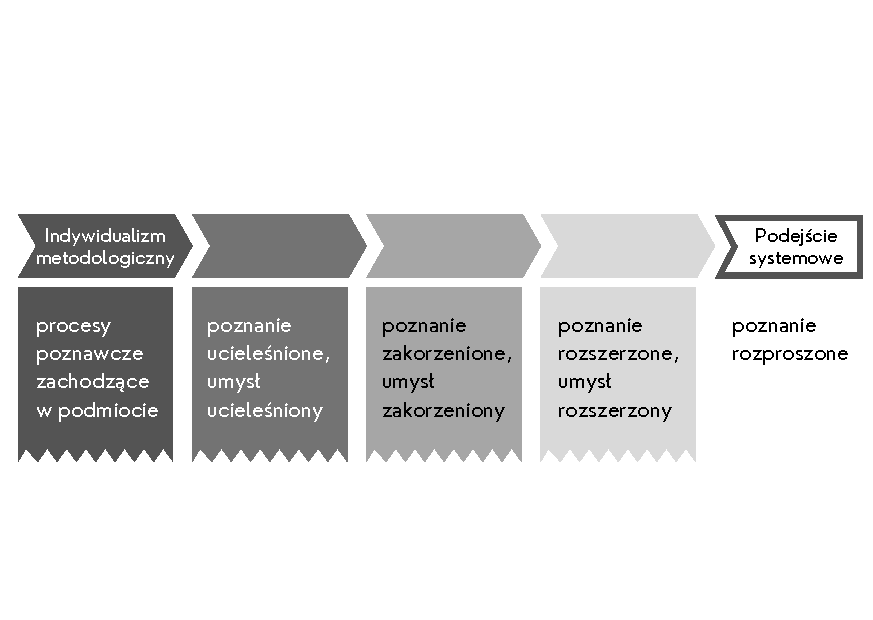
\includegraphics[width=1\textwidth]{ART_milkowski/ilustracja2pu.pdf}
\end{center}
 \caption{Różne stopnie odejścia od indywidualizmu metodologicznego.}\label{fig2milk}
\end{figure}



Dla Hutchinsa każdy taki system jest rozproszonym systemem poznawczym, niezależnie od jego skali -- ta bowiem może ulegać zmianie w~działaniu, a~przez to również przesuwać swoje granice. Poznanie rozproszone nie stanowi żadnego określonego rodzaju poznania, lecz ujęcie bądź sposób badania poznania każdego rodzaju: ,,Dla każdego procesu poznawczego musi istnieć sposób ujęcia go jako rozproszonego''. Dlatego ,,podejście to nie wnosi żadnych twierdzeń o~naturze świata. Jest raczej sposobem patrzenia na ten świat''
%\label{ref:RND1x6mwGwhCQ}(Hutchins, 2014, s.~36).
\parencite[][s.~36]{hutchins_cultural_2014}. %
 W~omawianej teorii właściwe pytania nie dotyczą więc tego, czy dane poznanie jest, czy nie jest rozproszone, ale składników danego systemu i~relacji między nimi, wyłaniania się procesów poznawczych z~interakcji w~systemie itp. Jak podkreśla badacz, perspektywa poznania rozproszonego nie ma żadnych założeń empirycznych. Nie można jej potwierdzić ani obalić. Można natomiast w~jej obrębie stawiać hipotezy empiryczne, między innymi hipotezę umysłu rozszerzonego, którą powinno się móc uzasadnić bądź odrzucić w~trakcie badań empirycznych 
%\label{ref:RNDSfUBAPgJSP}(Hutchins, 2014, s.~36–37).
\parencite[][s.~36–37]{hutchins_cultural_2014}.%


Warto zatem porównać teorię Hutchinsa z~koncepcją umysłu rozszerzonego
%\label{ref:RNDdjlTvhdZZj}(Clark, Chalmers, 2008).
\parencite[][]{clark_umysl_2008}. %
 Koncepcja ta głosi, że granice umysłu nie kończą się na głowie: częścią (a nie tylko narzędziem) umysłu mogą być zewnętrzne wobec układu nerwowego procesy i~przedmioty fizyczne, np. implanty stanowiące dodatkowe receptory zmysłowe, urządzenia obliczeniowe, systemy symboliczne (np. notacja matematyczna) lub nawet całe współpracujące ze sobą grupy. Badacz potwierdza pewne podobieństwa między nimi; podkreśla jednak dwie ważne różnice. Po pierwsze, koncepcja Clarka i~Chalmersa dotyczy tylko pewnego rodzaju poznania: w~jej ujęciu umysł czasami rozszerza się poza granice mózgu, a~czasami nie. Po drugie, w~systemie umysłu rozszerzonego daje się wyróżnić jego centrum (zwykle mózg lub też cały organizm). Dlatego też koncepcję tę można traktować jako dotyczącą szczególnego przypadku funkcjonowania umysłu -- czyli może ona być rozwijana na podstawie szerszych założeń teorii poznania rozproszonego 
%\label{ref:RNDe3LweFYY91}(Hutchins, 2011, s.~437–446, 2014, s.~35–36).
\parencites[][s.~437–446]{hutchins_enculturating_2011}[][s.~35–36]{hutchins_cultural_2014}.%


Hutchins, odrzucając indywidualizm metodologiczny, nie odchodzi od założeń komputacjonistycznych i~reprezentacjonistycznych, gdy określa poznanie jako obliczanie realizowane poprzez wytwarzanie, przetwarzanie i~przekazywanie stanów reprezentacyjnych
%\label{ref:RND4ffDHPRKLP}(Hutchins, 1995a, s.~49).
\parencite[][s.~49]{hutchins_cognition_1995}. %
 Przez ,,stany reprezentacyjne'' rozumie się stany nośników materialnych (zewnętrznych lub np. mózgowych), które oznaczają lub opisują przedmioty procesów poznawczych. Jednak zakres, jaki Hutchins przypisuje poznawczym reprezentacjom i~poznawczym procesom obliczeniowym, zdecydowanie wybiega -- na mocy głównego założenia jego teorii -- poza granice tradycyjnie rozumianych systemów poznawczych. Przedstawiana przez niego perspektywa przypomina nieco punkt widzenia Guliwera, którym byłby psycholog poznawczy, w~krainie olbrzymów: oto otrzymuje on wręcz wymarzoną możliwość bezpośredniej obserwacji procesów przebiegających w~systemie poznawczym w~makroskali, a~więc nie ,,w głowie'', lecz w~otoczeniu, w~które może wejść. Reprezentacje poznawcze stają się więc widzialne i~namacalne: mogą być nimi artefakty. Przez ,,artefakty poznawcze'' teoretycy poznania rozproszonego rozumieją obiekty, które służą do ,,przechowywania, udostępniania lub przetwarzania informacji na potrzeby funkcji reprezentowania, wpływając na poziom wykonania procesów poznawczych u~ludzi'' 
%\label{ref:RNDCkK0TYrHg7}(Norman, 1991, s.~11).
\parencite[][s.~11]{norman_cognitive_1991}. %
 Warto pamiętać, że artefaktami poznawczymi są również gesty czy wypowiedzi. Podobnie dostępne i~obserwowalne jest ich wytwarzanie, przetwarzanie i~przekazywanie, niekiedy dosłownie z~rąk do rąk 
%\label{ref:RND1cj0sn9xl2}(Hutchins, 1995a, s.~128–129).
\parencite[][s.~128–129]{hutchins_cognition_1995}. %
 Tym samym taki makrosystem poznawczy ma własne systemy pamięci zewnętrznej, jak i~mechanizmy oceny i~kontroli sytuacji, z~których żadne nie daje się sprowadzić do pamięci ani aktów oceny i~kontroli indywidualnych podmiotów poznania. Są one natomiast ,,rozproszone'', czy też rozdzielone między ludźmi w~kooperującej grupie lub artefaktami.

Perspektywa poznania rozproszonego to nie po prostu rozwinięcie kognitywistycznej historii o~sprzężeniu podmiotu poznawczego z~otoczeniem. Z~drugiej strony -- powtarzające się odwołania Hutchinsa do obiektów na różnych skalach czasoprzestrzennych, takich jak mózg, układ nerwowy czy ciało jednostkowego podmiotu ludzkiego, dobitnie pokazują, że stanowiska badacza nie można sprowadzać do eksternalistycznych, a~niekiedy wręcz ,,neurofobicznych'', ujęć organizacji systemów rozwiązywania problemów, którego modelowym przykładem miałoby być klasyczne studium nawigacji morskiej. Do takich wniosków mógł prowokować deklarowany przezeń we wcześniejszych pracach częściowy agnostycyzm co do możliwości badania wewnętrznych procesów umysłowych, który z~biegiem czasu coraz bardziej redukował\footnote{Szczegółowa rekonstrukcja w
%\label{ref:RNDc9IGnIMceq}(Afeltowicz, 2012, s.~178–188; Afeltowicz, Wachowski, 2015).
\parencites[][s.~178–188]{afeltowicz_modele_2012}[][]{afeltowicz_how_2015}.%
} -- choć trudno posądzać Hutchinsa o~ignorowanie wagi sprzężenia poznawczego między wewnętrznymi i~zewnętrznymi procesami poznawczymi, o~czym świadczy chociażby wnikliwa analiza funkcjonowania systemu kokpitu samolotu 
%\label{ref:RNDtxxt2Fkllo}(zob. Hutchins, 1995b; Hutchins, Klausen, 1996).
\parencites[zob.][]{hutchins_how_1995}[][]{engestrom_distributed_1996}. %
 Z~drugiej strony nie brakowało wyważonych ujęć jego teorii również we wcześniejszym okresie, jak chociażby autorstwa Yvonne Rogers 
%\label{ref:RND4byZChM8wV}(1997)
\parencite*[][]{rogers_brief_1997} %
 czy też takich współpracowników Hutchinsa, jak David Kirsh 
%\label{ref:RNDBuTbdSizkw}(1999).
\parencite*[][]{kirsh_distributed_1999}. %
 Jednak nie bez znaczenia są też odniesienia do koncepcji Latoura, przeciwnika uwzględniania jednostkowej psychologii w~wyjaśnianiach funkcjonowania kolektywnych struktur poznawczych, jak również twórcy podejścia metodologicznego, kojarzonego z~podejściem reprezentantów nurtu społecznych badań nad nauką i~techniką 
%\label{ref:RNDoko8d9fvmf}(zob. np. Hess, 2001).
\parencite[zob. np.][]{hess_ethnography_2001}.%


Główna metoda badawcza Hutchinsa jest etnograficzna. W~metodach etnograficznych docenia Hutchins możliwość badań nad rzeczywistym poznaniem w~rzeczywistym świecie, pozwalającą na wyprowadzenie ich poza ograniczoną przestrzeń laboratorium
%\label{ref:RNDwjlRdGES2W}(Hutchins, 2014, s.~43).
\parencite[][s.~43]{hutchins_cultural_2014}. %
 Takie podejście, zastosowane do procesów poznawczych, wydaje się w~pełni legitymizować odejście od indywidualizmu metodologicznego, nie tak oczywiste w~kognitywistyce. Jakościowa metoda etnograficznych badań poznawczych wykorzystuje obserwacje funkcjonowania danej wspólnoty do analiz jej aktywności poznawczej.

Różnicę między etnografią tradycyjną a~poznawczą można za Robertem Williamsem określić następująco: podczas gdy pierwsza zajmuje się znaczeniami wytwarzanymi przez członków danej wspólnoty kulturowej, druga koncentruje się na tym, jak te znaczenia są przez nich wytwarzane. Etnografowie tradycyjni wskazują materialne i~konceptualne zasoby składające się na lokalną rzeczywistość danej grupy, etnografowie kognitywni badają sposób, w~jaki te zasoby są wykorzystywane w~aktywności kulturowej. Pierwsi analizują myślenie ludzi definiujące ich grupę kulturową, natomiast drudzy obserwują sam ten proces; pierwsi opisują wiedzę, a~drudzy -- procesy konstrukcji i~wykorzystywania wiedzy. Oczywiście różnice te nie świadczą o~istnieniu między nimi przepaści
%\label{ref:RNDTBswyeN3Lq}(Williams, 2006, s.~838).
\parencite[][s.~838]{williams_using_2006}.%


Co tutaj istotne, zainteresowanie procesami poznawczymi funkcjonującymi w~środowisku naturalnym (tytułowe \textit{in the wild}) nie oznacza, że dla Huchinsa procesy przebiegające w~warunkach laboratoryjnych są nienaturalne i~niegodne badania lub że wręcz stoją poza kulturą. Nic bardziej błędnego: poznanie nie zna próżni kulturowej, więc miejsca, w~których przeprowadza się wyizolowane eksperymenty, nie mogą stanowić tutaj wyjątku. Obserwacje etnograficzne w~laboratoriach są po prostu trudniejsze, bo aspekty kulturowe pozostają tam niejako przezroczyste, co wymaga po prostu szczególnego podejścia badawczego
%\label{ref:RND3JRJN8V6Nn}(Hutchins, 1996, s.~66–67).
\parencite[][s.~66–67]{hutchins_response_1996}. %
 Że są możliwe i~interesujące, sam Hutchins udowadnia między innymi we współautorskim studium etnograficznym aktywności neurobadaczy 
%\label{ref:RNDkeP7sxcfO1}(Alač, Hutchins, 2004).
\parencite[][]{alac_i_2004}.%


Przedmiotem badań nad poznaniem rozproszonym ma być ,,natura poznania'' w~różnego rodzaju systemach działalności. W~badaniach Hutchinsa były one dość różnorodne, a~więc kultura Wysp Trobriandzkich, systemy nawigacji i~awiacji, społeczności małp człekokształtnych oraz delfinów, systemy interakcji człowiek-komputer (HCI), wspólnoty naukowców, jak również grupy realizujące tak codzienne praktyki kulturowe, jak opisana już kolejka. Poza obserwacjami \textit{in the wild} badacz ten przeprowadzał również obliczeniowe symulacje procesów kulturowych. Wskazując przy tym na różne skale realnych rozproszonych systemów poznawczych, plasuje on umysł rozszerzony na średnim poziomie skali, podkreślając, że w~systemie tego typu mamy do czynienia z~centralizacją poznawczą
%\label{ref:RNDYENpyx0zDM}(Hutchins, 2014, s.~37).
\parencite[][s.~37]{hutchins_cultural_2014}. %
 Systemami pozbawionymi takiej centralizacji byłyby już takie funkcjonalne struktury człowiek-artefakt, jak kokpity pojazdów, laboratoria, instytucje finansowe czy internet. Istnieją także rozległe i~różnorodne przestrzenie inteligencji zbiorowej, gdzie jednostkami systemu są samodzielne, aktywne podmioty poznania. Tutaj przykładem mogą być społeczności owadów, rynki ekonomiczne oraz media społecznościowe 
%\label{ref:RNDo452cepHYt}(Hutchins, 2014, s.~37).
\parencite[][s.~37]{hutchins_cultural_2014}.%


Przyjrzyjmy się najbardziej znanemu Hutchinsowskiemu studium przypadku, jakim były czteromiesięczne badania etnograficzne na początku lat dziewięćdziesiątych XX w. nad nawigacją morską na pokładzie amerykańskiego lotniskowca\footnote{Literatura przedmiotu obejmuje również prace poświęcone poznaniu rozproszonemu społecznie, które można by traktować jako pewnego rodzaju formę przejściową w~stosunku do analiz heterogenicznych struktur dokonywanych przez Hutchinsa
%\label{ref:RND7tkMcbcoey}(Roberts, 1964; Salomon, 1993).
\parencites[][]{roberts_self-management_1964}[][]{salomon_distributed_1993}. %
 }. Zespół marynarzy i~oficerów musi odpowiedzieć na prosto brzmiące pytanie: ,,gdzie jesteśmy i~dokąd zmierzamy?'', stawiane oczywiście z~perspektywy osób przebywających na pokładzie statku. Zapomnijmy tutaj na moment o~GPS i~systemach satelitarnych, ponieważ dopiero zaczynano je wdrażać i~były jeszcze dość zawodne.

Aby dokładnie wytyczyć położenie statku, nawigatorzy muszą dysponować co najmniej trzema łukami pozycyjnymi (AOP), wyznaczanymi na podstawie odległości do określonego punktu orientacyjnego, bądź liniami pozycyjnymi (LOP), wyznaczanymi na podstawie mierzonego w~stopniach położenia okrętu względem widocznego punktu orientacyjnego. Owe łuki i~linie oznaczane są na mapie cyrklem oraz specjalnym kątomierzem. Natomiast wyznaczanie LOP odbywa się z~wykorzystaniem pelorusów, czyli specjalnych urządzeń przypominających kompasy bez igły, umieszczonych na burcie lub pokładzie, dzięki którym obsługujący je marynarze wyszukują punkt obserwacyjny i~w żądanym momencie podają kwatermistrzowi odczyt z~tarczy. Najważniejszym przyrządem -- określanym przez Hutchinsa jako analogowy komputer -- jest mapa rozłożona w~kabinie nawigacyjnej, gdyż to wokół niej koncentrują się działania nawigatorów. Reprezentując przestrzeń geograficzną, daje ona nawigatorom unikatową perspektywę. Ponadto jednak mapa nawigacyjna stanowi urządzenie obliczeniowe: dzięki niej zachodzi zewnętrzne obliczanie, niemające odpowiednika w~niczyjej obecnej tam głowie, nawet oficerów. Odpowiedzi na zadawane pytania nawigatorzy otrzymują, wykonując proste czynności takie jak obsługa cyrkla i~kątomierza, rysowanie linii czy przepisywanie cyfr. Cała procedura stanowi, zdaniem Hutchinsa, doskonałą ilustrację Latourowego myślenia za pomocą rąk i~oczu
%\label{ref:RNDMaCVn4m2rV}(Hutchins, 1995a, s.~142–143).
\parencite[][s.~142–143]{hutchins_cognition_1995}. %
 W~tym kontekście Hutchins przytacza słowa Herberta Simona: ,,rozwiązanie problemu to po prostu przedstawienie go w~taki sposób, aby rozwiązanie stało się oczywiste'' 
%\label{ref:RNDHN1L3EqIMz}(Hutchins, 1995a, s.~117).
\parencite[][s.~117]{hutchins_cognition_1995}.%


Mapa nawigacyjna pełni kilka ważnych funkcji. Stanowi podstawową reprezentację zewnętrzną, umożliwiającą przeprowadzanie obliczeń. Pozwala na integrowanie i~porównywanie informacji pochodzących z~różnych źródeł. Służy do koordynacji ludzkich działań. Stanowi także środek monitorowania jakości pracy nawigatorów. Przy tym wszystkim jest zewnętrznym systemem pamięci (zresztą przechowywanym pieczołowicie i~w kilku kopiach), obejmującym wiedzę (wraz z~jej modyfikacjami) zarówno członków danej załogi okrętu, jak i~różnych pokoleń marynarzy, badaczy, geografów, kartografów
%\label{ref:RNDKwGI4POv2k}(Afeltowicz, Wachowski, 2015, s.~93–98; Hutchins, 1995a, s.~61–143).
\parencites[][s.~93–98]{afeltowicz_how_2015}[][s.~61–143]{hutchins_cognition_1995}.%


\section{Korzenie, inspiracje, interpretacje}

Do jakiego stopnia mamy tutaj do czynienia z~nową propozycją teoretyczną? Jak się mają te badania nad poznaniem do reszty nauk poznawczych? Odpowiedzi na oba te ważne pytania wiążą się ze sobą, a~wstępną odpowiedź naszkicowaliśmy już wcześniej, omawiając ekologię poznawczą.

Osbeck i~Nersessian
%\label{ref:RNDJbap64ket5}(2014),
\parencite*[][]{osbeck_situating_2014}, %
 podejmując własną próbę historycznego usytuowania teorii poznania rozproszonego, wskazują na analogie z~psychologią funkcjonalną -- w~tym stanowiskami Williama Jamesa i~Johna Deweya -- jednocześnie sugerując związki teoretyczne z~pragmatyzmem filozoficznym. Funkcjonaliści podejmowali ,,problem kontekstu'', ujmując działający podmiot w~,,pełnej'' sytuacji, jego życie umysłowe jako proces adaptacyjny, a~procesy poznawcze raczej jako pewną aktywność niż nabywanie wiedzy. Porównując psychologię funkcjonalną i~teorię poznania rozproszonego, Osbeck i~Nersessian wskazują na zbieżności: perspektywa systemowa i~dynamiczna, nacisk na rozwiązywanie problemów, sprzeciw wobec czysto intelektualnej wizji poznania, oddzielonego od świata rzeczy i~zjawisk społecznych, preferowanie badań nad zjawiskami zachodzącymi w~rzeczywistym (a nie sztucznym, laboratoryjnym) środowisku.

Na uwagę zasługują wpływy i~zbieżności z~perspektywą radzieckiej szkoły kulturowo-historycznej Lwa Wygotskiego i~Aleksandra Łurii. Ten ostatni, komentując stanowisko Wygotskiego
%\label{ref:RND34bUoj8PY6}(np. Vygotskij, 1971; warto także porównać z: Mead, 1975),
\parencites[np.][]{vygotskij_wybrane_1971}[warto także porównać z:][]{mead_umysl_1975}, %
 wywodzącego indywidualne akty psychiczne z~zachowań grupowych, stwierdzał, że jeśli mamy wyjaśnić złożone formy ludzkiej świadomości, powinniśmy w~analizach wyjść poza granice organizmu, w~sferę zewnętrznych warunków jego życia, uwzględniając tak społeczny, jak i~historyczny ich wymiar 
%\label{ref:RNDaAnLjhFbmJ}(Luriâ, 1979).
\parencite[][]{luria_azyk_1979}. %
 Michael Cole i~Yrjö Engeström wymieniają następujące elementy podejścia kulturowo-historycznego, które można traktować jako początki teorii poznania rozproszonego: zasady rządzące ,,naturalnymi'' psychicznymi czynnościami człowieka są różne od zasad rządzących jego czynnościami ,,kulturowymi'' -- upośrednionymi przez narzędzia i~normy społeczne; to kulturowe upośrednienie kształtuje szczególnego rodzaju strukturę ludzkiego umysłu i~zachowania, modyfikując podmiot i~jednocześnie jego otoczenie; interakcję między nimi regulują kulturowe artefakty, zarówno materialne, jak i~symboliczne. Niezwykle ważnym narzędziem tego upośrednienia jest język. W~danym otoczeniu kulturowym skumulowana jest również wiedza poprzednich pokoleń, dlatego w~rozwoju osobniczym ważną rolę odgrywa środowisko społeczne. Stąd też naturalną jednostką analizy w~badaniach nad ludzkim zachowaniem stają się systemy czynności, rozumiane jako historycznie uwarunkowane systemy relacji między jednostkami ludzkimi a~ich najbliższym, kulturowo ustrukturyzowanym otoczeniem. Autorzy zestawiają wyniki prac radzieckich psychologów nurtu kulturowo-historycznego z~wnioskami wspomnianego już Deweya, ale także Wilhelma Wundta i~Hugo Münsterberga, dostrzegając w~nich zbliżone sposoby konceptualizacji poznania jako zjawiska rozproszonego, w~ramach których dochodzi do zjednoczenia nauk przyrodniczych i~kulturowych 
%\label{ref:RNDxtyiUJ6lJK}(Cole, Engeström, 1993).
\parencite[][]{cole_cultural-historical_1993}.%


Dysponujemy już pewną wiedzą o~stosunkowym nowatorstwie teorii Hutchinsa, powróćmy więc do pytania o~to, jak ma się ona do szerszego dorobku nauk poznawczych. O~stopniu osadzenia teorii poznania rozproszonego w~klasycznej kognitywistyce dobre pojęcie daje książka \textit{Cognition in the Wild}. Uwidacznia się to między innymi w~specyficznym rozumieniu obliczania i~reprezentacji: choć sama przyjmowana przez tego autora definicja poznania -- czyli (przypomnijmy) obliczania realizowanego poprzez wytwarzanie, przetwarzanie i~przekazywanie stanów reprezentacyjnych -- bezkolizyjnie łączy omawianą perspektywę z~klasycznymi podejściami w~naukach poznawczych, to wątpliwości pojawiają się co do zakresu, jaki Hutchins przypisuje pojęciom reprezentacji oraz procesom obliczeniowym. Trudno bowiem uznać reprezentacje zewnętrzne (znaki, ilustracje czy gesty) za po prostu równoważne wewnętrznym reprezentacjom umysłowym. Podobnie brakuje powszechnej zgody na to, by uznać zbiorową czynność kolektywu współpracującego przy rozwiązywaniu wspólnego problemu, za czynność poznawczą.

Autor \textit{Cognition in the Wild} wskazuje na pewne nieporozumienia związane z~pojęciami stosowanymi w~kognitywistyce, a~także postuluje reinterpretację jej historii. U~podstaw nieporozumień -- historycznie wzmocnionych -- leży, jego zdaniem, podstawowe niezrozumienie podobieństw i~różnic między komputerami a~umysłami.

Dla Hutchinsa idea procesu obliczeniowego jest podstawowa nie tylko dla poznania, lecz także kultury; opanowanie systemów formalnych to wręcz klucz do rozumienia nowoczesnej cywilizacji
%\label{ref:RNDLR48tqgRIS}(Hutchins, 1995a, s.~359–360).
\parencite[][s.~359–360]{hutchins_cognition_1995}. %
 Jednak to nie umysł ludzki, ile większy wycinek ludzkiego świata kulturowego miałby być komputerem: ,,Architektura systemu fizycznych symboli nie stanowi modelu indywidualnego poznania, ale model działania systemu społeczno-kulturowego, z~którego usunięto indywidualny ludzki podmiot'' 
%\label{ref:RNDP3BxoM3qkK}(Hutchins, 1995a, s.~363).
\parencite[][s.~363]{hutchins_cognition_1995}. %
 Analogicznie Hutchins traktuje system Searle'owskiego chińskiego pokoju jako społeczno-kulturowy system poznawczy, którego właściwości wykraczają poza możliwości poznawcze ludzkiej jednostki. Searle przedstawia następujący eksperyment myślowy 
%\label{ref:RNDw5VUtfF02C}(Searle, 1995).
\parencite[][]{searle_umysly_1995}. %
 W~pewnym pomieszczeniu -- zwanym ,,chińskim pokojem'' -- znajduje się człowiek, posługujący się skomplikowanym podręcznikiem przekładu z~języka chińskiego na angielski. Sam jednak w~ogóle nie zna chińskiego. Przez otwór do pokoju dostaje pytanie w~języku chińskim. Korzystając z~angielskiego podręcznika i~wertując go, odpowiada na pytanie, też po chińsku. Czy powiedzielibyśmy, że rozumie po chińsku? Nie! Dlatego też, powiada Searle, nie ma podstaw, aby przypisywać komputerom rozumienie języka naturalnego. Searle jednak nie rozpoznaje złożoności rozproszonego systemu poznawczego, który sam opisuje w~swoim eksperymencie myślowym. Podobnie, zgodnie z~fałszywą (zdaniem Hutchinsa) ideą, że komputer wykonany jest na obraz i~podobieństwo człowieka, dziesiątki lat historii kognitywistyki można postrzegać jako dążenie do przerobienia obrazu człowieka na obraz komputera 
%\label{ref:RNDkYZeMM4ccG}(Hutchins, 1995a, s.~361–363).
\parencite[][s.~361–363]{hutchins_cognition_1995}. %
 Przy takim podejściu ciało, emocje, kultura musiały stać się elementami dodanymi, uwzględnianymi dopiero na późniejszym etapie dociekań.

Autor \textit{Cognition in the Wild} zakłada, że ludzie rzeczywiście przetwarzają wewnętrzne reprezentacje symboli. Ale nie wierzy w~to, by to manipulacja symbolami stanowiła istotę indywidualnego poznania. Pylyshynowi, który opisuje manipulowanie symbolami zakodowanymi w~koralikach liczydła
%\label{ref:RNDMFKcdNi2s5}(Pylyshyn, 1989, s.~56),
\parencite[][s.~56]{pylyshyn_computing_1989}, %
 Hutchins zarzuca zignorowanie tego, co robi liczący, abstrahowanie od funkcji jego rąk i~oczu, od istoty samego uczenia się, na rzecz skupienia się na właściwościach systemu, który wyłania się dzięki aktywności osoby manipulującej koralikami. Oczywiście Pylyshyn dobrze opisuje obliczeniowe właściwości systemu społeczno-kulturowego, lecz nie aktywność poznawczą podmiotu ludzkiego. Hutchins domaga się podejścia ucieleśnionego, to znaczy uwzględniającego konkretny, fizyczny udział osobnika w~czynnościach liczenia i~uczenia się, gdyż dopiero wtedy można mówić o~jego użytkowaniu przyrządu do rozwiązywania problemów oraz o~nabywaniu określonych umiejętności. W~tych dociekaniach konieczne jest usytuowanie podmiotu poznającego w~realnym świecie. Hutchins przyznaje, że klasyczni zwolennicy hipotezy \textit{systemu fizycznych symboli} są tego świadomi. Allen Newell i~Herbert Simon potwierdzają istotność tak zwanych pamięci zewnętrznych -- a~więc materialnych zasobów dostępnych w~otoczeniu podmiotu rozwiązującego dany problem poznawczy i~wykorzystywanych przezeń równolegle z~pamięcią wewnętrzną 
%\label{ref:RNDBqDSyMdOeS}(Newell, Simon, 1972, s.~800–803).
\parencite[][s.~800–803]{newell_human_1972}. %
 Badacz dostrzega dobry punkt wyjścia, zauważa jednak, że przez dziesiątki lat od wydania przytaczanej tu książki Newella i~Simona wykorzystanie materialnych struktur otoczenia w~procesach poznawczych jakoś nie interesowało głównego nurtu kognitywistyki 
%\label{ref:RNDcRwZJasC4s}(Dahlbäck, Kristiansson, 2016; Hutchins, 1995a, s.~364–370).
\parencites[][]{dahlback_perspective_2016}[][s.~364–370]{hutchins_cognition_1995}.%


Badania Hutchinsa wpisują się w~dosyć swoiście pojmowaną naturalizację badań społecznych -- a~mianowicie pozwalają spełnić wymóg naturalizmu metodologicznego, głoszący, że w~badaniach empirycznych
%metody badawcze
dopuszczalne są wszystkie i~tylko te metody, które są typowe dla nauk przyrodniczych. Za taką naukę przyrodniczą uchodzić ma, rzecz jasna, antropologia kognitywna, integrująca się również z~pozostałymi elementami konglomeratu kognitywistycznego, w~tym także do pewnego stopnia z~neuronauką w~ramach neuroantropologii
%\label{ref:RNDmCjTTYm6pd}(Lende, Downey, 2012).
\parencite[][]{lende_encultured_2012}. %
 Jest tak dlatego, że Hutchins bardzo swoiście rozumie też antropologię poznawczą: jest ona mianowicie badaniem kultury metodami, które proponowano do wyjaśniania procesów rozwiązywania problemów w~psychologii poznawczej. Te wyjaśnienia odwołują się m.in. do operowania symbolami.

Hutchins odwołuje się do bardzo wpływowej propozycji metodologicznej, sformułowanej przez Davida Marra
%\label{ref:RNDytVMerjGC8}(1982),
\parencite*[][]{marr_vision_1982}, %
 a~powszechnie przyjmowanej w~badaniach kognitywistycznych. Marr uważał, że systemy obliczeniowe należy wyjaśniać na trzech poziomach ich realizacji, ponieważ dopiero wyjaśnienie wszystkich poziomów jest kompletne i~satysfakcjonujące. Przede wszystkim należy wiedzieć, jakie zadanie -- opisywane w~kategoriach przetwarzania informacji -- realizuje dany system i~dlaczego realizacja tego zadania jest właściwa w~danym otoczeniu. Ten poziom Marr zwał ,,obliczeniowym'', lecz jest to termin nieco mylący; inni stosowali określenia ,,poziom wiedzy'' 
%\label{ref:RND3bcrtgwcDH}(Newell, 1981)
\parencite[][]{newell_knowledge_1981} %
 ,,poziom semantyczny'' 
%\label{ref:RNDor3Z8HGaA2}(Pylyshyn, 1984)
\parencite[][]{pylyshyn_computation_1984} %
 lub ,,ekologiczny'' 
%\label{ref:RNDHJjKtYSxCi}(Sterelny, 1990).
\parencite[][]{sterelny_representational_1990}. %
 W~przypadku określenia położenia statku wejściowe informacje dostępne są z~wielu, często dających rozbieżne wyniki, przyrządów pomiarowych, których obsługa wymaga współdziałania wielu osób. Rozwiązaniem ma być niezbędna w~żegludze para współrzędnych nałożona na mapę.

Na drugim poziomie -- kluczowym dla Marra -- opisuje się algorytmy i~reprezentacje, na których owe algorytmy pracują. Innymi słowy, opisuje się system obliczeniowy jako urzeczywistniający precyzyjnie opisane procesy przetwarzania informacji, których postać jest dokładnie określona. Tu Hutchins abstrakcyjnie opisuje strukturę systemu -- odzwierciedlającą podział pracy poznawczej -- i~poszczególne składowe reprezentacje oraz kanały przesyłania informacji (np. telefon na pokładzie).

Na trzecim zaś poziomie Marr domaga się wskazania realizacji sprzętowej danego systemu obliczeniowego. Hutchins wskazuje w~szczególności na ograniczenia materialne interakcji społecznej, dzięki którym działania są lepiej koordynowane, a~sekwencja działań mająca prowadzić do ustalenia położenia w~danym momencie jest wykonywana bez zakłóceń. Pozostaje on w~dużej mierze neutralny w~sprawie tego, jak mają się działania poszczególnych osób, będących częściami dużego, rozproszonego systemu poznawczego, do ich indywidualnych zdolności poznawczych. Uważa, że właściwe wyjaśnienie systemu rozproszonego nie musi schodzić na taki niższy poziom, a~zjawisko można wyjaśnić trafnie na bardziej abstrakcyjnym poziomie opisu struktury społeczno-kulturowej wraz z~jej materialną realizacją.

Przy takim podejściu widać od razu, że Hutchins korzysta z~narzędzia, które pozwala mu modelować podział pracy poznawczej, i~to także z~uwzględnieniem skuteczności tej pracy. W~tym miejscu tematyka jego prac wprost łączy się z~klasycznym wątkiem badań socjologicznych, a~metoda badawcza -- opis antropologiczny -- zbliża go do badań społecznych prowadzonych w~mikroskali, lecz jednocześnie metodami umożliwiającymi matematyzację. Tu Hutchins różni się też od innych antropologów poznawczych, którzy, w~odróżnieniu od większości kognitywistów korzystających w~ogromnej mierze z~modelowania obliczeniowego, rzadko odwołują się do symulacji komputerowych, a~prawie nigdy nie przeprowadzają symulacji realnych procesów społeczno-poznawczych w~celu ich wyjaśniania i~przewidywania.

Hutchins między innymi opracował symulacje zjawiska zwanego ,,błędem potwierdzania''. Polega ono na tym, że skłonni jesteśmy uznawać za prawdziwą tę informację, która potwierdzałyby wcześniejsze założenia lub oczekiwania. Badacz pokazał, że zjawisko to może zachodzić w~grupie w~formie procesu rozproszonego; wykorzystał w~tym celu sieć koneksjonistyczną zwaną ,,siecią spełniania ograniczeń'', uzyskując uproszczony model grupowej interakcji. Przy okazji zaobserwował, że błąd potwierdzania zachodzi tym słabiej, im większa jest komunikacja (interakcja) między jednostkami w~sieci
%\label{ref:RNDHhYhoRT1qF}(Hutchins, 1995a, s.~239–255).
\parencite[][s.~239–255]{hutchins_cognition_1995}.%


Podział pracy poznawczej stanowi istotę działania wielu organizacji i~instytucji społecznych, a~próby udoskonalenia ich działania -- jeśli same nie adaptują się do otoczenia -- mogą z~pewnością skorzystać z~bardziej kognitywnego podejścia. Dzięki zastosowanemu tutaj podejściu Hutchinsa można opisać przebieg procesu przetwarzania informacji i~przeanalizować jego efektywność ze względu na założony cel poznawczy. Możliwa jest więc poznawcza analiza społecznych procesów podejmowania decyzji, tak politycznych, jak i~naukowych czy potocznych.

Nie oznacza to wszelako, że metoda obrana przez Hutchinsa jest idealna. Metodologia Marra została opisana przezeń jedynie we wstępie metodologicznym do jego wpływowej książki i~nie odzwierciedla zacierania się granic między kognitywistyką a~neurokognitywistyką, a~także między badaniem procesów kulturowych i~poznawczych. Badacze interesują się bowiem często tym, jakie mechanizmy odpowiadają za procesy psychiczne i~starają się zawęzić swoje hipotezy, odwołując się do świadectw neurobiologicznych czy kulturowych. Marr, \textit{notabene}, też tak czynił, kiedy zwracał uwagę na rozłączne pojawianie się pewnych zaburzeń poznawczych przy ogniskowych uszkodzeniach mózgu. Jednak co do zasady uważał, że nie jest to bynajmniej konieczny element metody wyjaśniania, a~jego opis poziomu realizacji sprzętowej (neuronalnej) pozostaje, podobnie nieco jak i~u~Hutchinsa, osobliwie nieprecyzyjny.

Skupienie się Hutchinsa na budowie i~morfologii systemów poznawczych na różnych poziomach ich podsystemów, a~przez to na udziale artefaktów w~ludzkich procesach poznawczych oraz ogólnie funkcjonowaniu ekosystemów kulturowych, wykazuje duży związek z~pracami Donalda Normana, zwłaszcza z~książką \textit{Things that Make us Smart}
%\label{ref:RNDMIEchfVLok}(1993).
\parencite*[][]{salomon_distributed_1993}. %
 Pojawia się w~niej zresztą pojęcie i~wyjaśnienie poznania rozproszonego oraz wyników badań Hutchinsa jeszcze przed publikacją \textit{Cognition in the Wild}.

Miejsce i~recepcja Normana w~kognitywistyce wymaga kilku słów wyjaśnienia. Ten amerykański kognitywista i~teoretyk wzornictwa przemysłowego, a~jednocześnie najbardziej chyba wpływowy badacz interakcji człowiek-komputer (HCI), jak i~szerzej: człowiek–artefakt, uprawia swoistą inżynierię poznawczą. Zainteresowany jest nie tyle rozwijaniem teorii znanych już interakcji człowiek–artefakt, ile projektowaniem tych interakcji, ich kulturowym zastosowaniem (i tym samym badaniem przez projektowanie). To nastawienie bardzo dobrze współgra z~równie praktyczną orientacją Hutchinsa, konsekwentnie odwołującego się do kulturowego wykorzystywania rzeczy.

\section{Szkodliwe moratorium}

Perspektywą najbardziej zbliżoną do perspektywy Hutchinsa jest nurt społecznych badań nad nauką i~techniką, reprezentowany między innymi przez Brunona Latoura, do którego prac Hutchins zresztą wyraźnie się odwoływał.

W~klasycznych naukach nad poznaniem i~mózgiem zagadnienia społeczne w~poznaniu sprowadza się zasadniczo do procesu społecznego wiązanego z~nabywaniem i~przetwarzaniem informacji o~innych ludziach, komunikowaniem się, empatią. Ścieżka analizy wiedzie tutaj od jednostkowych umysłów czy mózgów do społeczeństwa
%\label{ref:RND8XdzRJeEgZ}(zob. np. Fiske, Taylor, 2008).
\parencite[zob. np.][]{fiske_social_2008}.%


Tymczasem -- jak pokazują Ronald Giere i~Barton Moffatt -- perspektywa naukoznawcza ukazuje wspomnianą relację jako opozycję, w~pewnych przypadkach wskazując na dominację wymiaru społecznego, co byłoby pokłosiem socjologii wiedzy
%\label{ref:RNDGHooPYkgJU}(zob. także Brown, 2011; Giere, Moffatt, 2003, s.~301–302).
\parencites[zob. także][]{brown_science_2011}[][s.~301–302]{giere_distributed_2003}. %
 Wyzywającą manifestacją tej dominacji było dziesięcioletnie moratorium na odwoływanie się do umysłu w~wyjaśnianiu sukcesu nauki, które zaproponował Latour ze Steve'em Woolgarem. Rzucali oni wyzwanie kognitywistyce wyjaśniającej efektywność nauki przez odwołanie do umysłu, ujmowanego jeszcze w~sposób odcieleśniony i~oderwany od kontekstu społecznego i~materialnego: ,,My zaś w~tym miejscu obiecujemy, że jeśli pod koniec tego okresu zostanie cokolwiek [związanego z~poznaniem naukowym] do wyjaśnienia, to my także zwrócimy się w~stronę umysłu!'' 
%\label{ref:RNDQ8MYVWAXEp}(Latour, Woolgar, 2020, s.~366).
\parencite[][s.~366]{latour_zycie_2020}.%


W~badaniach nad poznaniem naukowym Hutchins wydawałby się doskonałym partnerem Latoura; wszak analizował czynności badaczy w~laboratorium neuronaukowym
%\label{ref:RNDq7az7dkeo7}(Alač, Hutchins, 2004).
\parencite[][]{alac_i_2004}. %
 Jego uwagi dotyczące wizualizacji naukowych wpisują się w~perspektywę Latoura 
%\label{ref:RNDQ0asW0EmjX}(np. Latour, 2012).
\parencite[np.][]{latour_wizualizacja_2012}. %
 Prześledźmy ich pouczający spór 
%\label{ref:RNDmhrfwswWJZ}(Latour, 1996; Hutchins, 1996).
\parencites[][]{latour_cogito_1996}[][]{engestrom_distributed_1996}.%


Latour jest badaczem społecznym i~filozofem nauki, kojarzonym z~konstruktywistyczną teorią aktora-sieci (ANT), która przypisuje sprawczość czynnikom ludzkim i~pozaludzkim, znajdującym się w~zmiennych (czasowo wzmacnianych lub też słabnących) sieciach relacji
%\label{ref:RND7AXCpLIIYs}(zob. np. Latour, 2010).
\parencite[zob. np.][]{latour_splatajac_2010}. %
 ,,W szesnastym wieku nie pojawił się żaden nowy człowiek, a~we współczesnych laboratoriach nie pracują wcale mutanci o~rozrośniętych mózgach'' -- stwierdza, namawiając do szukania przyczyn spektakularnych sukcesów nauki w~praktykach i~narzędziach badaczy 
%\label{ref:RNDPXBhMczGqs}(Latour, 2012, s.~208).
\parencite[][s.~208]{latour_wizualizacja_2012}. %
 Analogicznie Hutchins -- co nie uszło uwadze Latoura -- każe szukać źródeł ludzkich mocy poznawczych w~przetworzonym już otoczeniu i~użytkowanych artefaktach, krytykując popularne przekonanie o~zaawansowanej technice jako konsekwencji zaawansowanych zdolności poznawczych czy umysłów 
%\label{ref:RNDvCop10Yenj}(Hutchins, 1995a, s.~169, 355).
\parencite[][s.~169, 355]{hutchins_cognition_1995}.%


Latour dostrzega w~\textit{Cognition in the Wild} kompleksowe ujęcie praktyk poznawczych w~ich naturalnym kontekście. Hutchins pokazuje, jak owe praktyki mogą być dobrze skoordynowane, precyzyjne i~zdyscyplinowane, co pozwala na sformalizowaną analizę, mimo iż przeprowadzaną poza przestrzenią laboratorium. Badacz jawi się tutaj jako jeden z~antropologów (obok Jean Lave, Lucy Suchman czy Chucka Goodwina), którzy w~swojej karierze badali zarówno społeczności tradycyjne o~nisko zaawansowanej technice, jak i~silnie zmodernizowane. Przewaga Hutchinsa nad nim polega na wykorzystaniu formalnego rozumowania, metrologii i~matematyki. Latour docenia wagę i~radykalność głównej tezy książki, która w~jego ujęciu określa opisywane tam zjawisko poznania jako niemające ,,nic wspólnego z~umysłami czy jednostkami ludzkimi, lecz z~rozprzestrzenianiem reprezentacji przez różnorodne ośrodki, koordynowane przez dość słabo wyposażony ludzki podmiot działający w~grupie, w~ramach jakiejś kultury, z~wykorzystaniem artefaktów, mogący internalizować pewną część tego procesu''
%\label{ref:RNDISZWnbV0C5}(Latour, 1996, s.~56).
\parencite[][s.~56]{latour_cogito_1996}. %
 Według Latoura teza ta mogłaby zreformować całość nauk poznawczych. Jedna z~radykalnych zmian to przekierowanie uwagi z~umysłowych czy indywidualnych czynności na przebieg zmian reprezentacji. W~takich badaniach tracą znaczenie sformułowania typu ,,myślę'' lub ,,reprezentuję''; nie ma sensu pytać, co się dzieje w~umyśle kreślarza na statku podczas wykonywania zbiorowej pracy nawigacyjnej. Latour podkreśla konsekwencje tego odwrotu od zdarzeń umysłowych i~zwrotu ku ośrodkom: docenienie roli techniki i~zapośredniczających artefaktów, które nie służą wzmacnianiu ludzkich zdolności poznawczych, lecz odkrywaniu nowych problemów poznawczych.

Zdaniem Latoura, ,,pod skórą'' indywiduum przebiegają te same procesy, co na zewnątrz. Myślący podmiot stanowi dla Hutchinsa szczególnego rodzaju ośrodek umożliwiający koordynację wielu innych ośrodków, zewnętrznych, wewnętrznych, w~postaci artefaktów, idei czy relacji społecznych. W~stwierdzeniu tym Latour widzi ostateczny rozpad psychologii. Myślący podmiot przypomina tutaj coś w~rodzaju blatu biurka dobrze zorganizowanego menedżera: jest pusty, odkąd wszystko inne zostało oddelegowane na zewnątrz do czegoś lub kogoś innego
%\label{ref:RNDbzZJwmVlj2}(Latour, 1996, s.~59).
\parencite[][s.~59]{latour_cogito_1996}. %
 Nic więc dziwnego, że Latour z~aprobatą powtarza przekonanie Hutchinsa, że komputery, ,,ukochany model umysłu'' przedstawicieli klasycznej perspektywy, mogą podsuwać dobry opis funkcjonowania systemów społeczno-kulturowych, ale nie ludzkich procesów poznawczych.

Na tym aprobata Latoura się jednak kończy. Ku jego rozczarowaniu Hutchins okazuje się niekonsekwentny, liczy bowiem na psychologię lepiej ugruntowaną empirycznie -- podczas gdy, zdaniem Latoura, stara się ona jedynie wtłaczać kategorie poznawcze do indywidualnych umysłów obdarzonych świadomością i~odpowiedzialnością. Równie niepokojącą dla niego ideą przewijającą się przez książkę jest założenie, że po jednej stronie (tego, co dane) mamy świat, a~po drugiej zdolności poznawcze, co niekoniecznie zgadza się z~ideą rozproszenia (wedle Latoura). Hutchins pisze o~procedurze bezpośredniego uzgadniania mapy ze światem -- a~przecież operatorzy pelorusa uzgadniają nie świat z~mapą, tylko odczyty z~kompasu z~istniejącymi już punktami orientacyjnymi na mapie, w~czym istotną rolę odgrywają zapośredniczenia, o~których autor najwyraźniej tutaj zapomina
%\label{ref:RNDX1YRxstiI4}(Latour, 1996, s.~60).
\parencite[][s.~60]{latour_cogito_1996}.%


Latour walczy z~mitem wyższych zdolności poznawczych i~lepiej rozwiniętych cywilizacyjnie umysłów: ,,Myślą laboratoria, odkrywają wspólnoty, rozwijają się dziedziny, spostrzegają przyrządy, a~nie jednostkowe umysły''
%\label{ref:RNDD15Nlq6UZy}(Latour, 1996, s.~61).
\parencite[][s.~61]{latour_cogito_1996}. %
 Jego zdaniem, pogląd ten został już należycie wyrażony i~sprecyzowany przez naukoznawców, z~czego Hutchins nie zdaje sobie sprawy i~dlatego nie usuwa indywiduum z~pola widzenia w~poznaniu rozproszonym.

Hutchins w~odpowiedzi zauważa, że Latour chciałby rozpuścić indywidualny podmiot i~psychologię indywiduum. Sprzątnąć, wymieść to, co indywidualne, z~podmiotu, niczym z~biurka, jak w~przytoczonym wcześniej porównaniu. Twórca teorii aktora-sieci chciałby oddelegować wszystko ,,na zewnątrz do czegoś lub kogoś innego'' -- tylko kogo, skoro według niego żadnego podmiotu w~ogóle nie ma? Wbrew Latourowi ambicją Hutchinsa nie jest wyprzątnięcie wszystkiego z~podmiotu ludzkiego, tylko zespolenie tego, co w~nim, z~jego otoczeniem. Zdarzenia poznawcze muszą gdzieś się odbywać, a~częściowo odbywają się wewnątrz podmiotu. Choć fragment książki o~myślącym podmiocie jako specjalnym ośrodku koordynującym Latour przytacza na poparcie swojej wizji rozpuszczenia psychologii indywiduum, Hutchins stawia w~nim pytanie, jakiego rodzaju ośrodkiem jest myślące indywiduum -- na które odpowiedzią byłaby nowa, adekwatna do aktualnych wyzwań badawczych teoria psychologiczna. Dzięki niej umysł ujawni się nam nie jako ,,uprzątnięty'', lecz jako ,,umeblowany'' inaczej, niż wcześniej sądzono. A~kwestia, jak dobrze opisywać oraz modelować takie systemy, pozostaje trudna
%\label{ref:RND42T3C4oUfl}(Hutchins, 1996, s.~64–66, 68).
\parencite[][s.~64–66, 68]{hutchins_response_1996}.%


Jaki jest stosunek Latoura do interdycyplinarności, czy też szerzej~-- ,,wzajemnego oświecania się'' dyscyplin? Z~jednej strony, uderza on w~mit odrębnych, autonomicznych dyscyplin. Z~drugiej strony, nie najlepiej ocenia dotychczasowe (a więc podejmowane przed Hutchinsem) próby współpracy psychologii i~nauk społecznych, określając na przykład psychologię społeczną jako monstrum, które skupia to, co najgorsze, z~obu dyscyplin
%\label{ref:RNDloPJrlZkhU}(Latour, 1996, s.~58).
\parencite[][s.~58]{latour_cogito_1996}. %
 Nie można mu rzeczywiście odmówić, że na różne sposoby wyraża wsparcie dla zasypywania granic czy też likwidacji napięcia w~podejściach antropologii i~kognitywistyki, sprowadzające się do dylematu, czy poznanie jest konstytuowane przez kulturę, czy też jest od kultury niezależne. I~w tym kontekście zasadniczo komplementuje właśnie Hutchinsa za wyczulenie na ten problem i~pracę na rzecz uzgodnienia nauk przyrodniczo-ścisłych z~badaniami nad poznaniem ,,in the wild''. Recenzent \textit{Cognition in the Wild} chciałby bardzo, jak twierdzi, aby odnowiona antropologia poznawcza ,,współpracowała blisko z~tymi przedstawicielami nauk przyrodniczo-ścisłych, którzy mają takie same zainteresowania i~wielu tych samych wrogów'' 
%\label{ref:RNDMfywQqx6ZC}(Latour, 1996, s.~61).
\parencite[][s.~61]{latour_cogito_1996}. %
 Cóż z~tego jednak, skoro Latour wydaje się nie akceptować samego przyjmowanego w~kognitywistyce rozumienia tego, co poznawcze. Jego moratorium zaś miało być także wyrazem sprzeciwu wobec ,,luźnego i~łatwego'' podejścia epistemologów do wyjaśnień poznawczych 
%\label{ref:RNDc2BxdcWdGJ}(Latour, 1996, s.~62).
\parencite[][s.~62]{latour_cogito_1996}. %
 Innymi słowy, nie ma zgody Latoura na to, jak Hutchins rozumie dalej to, co jest przetwarzane obliczeniowo, z~jednego medium reprezentacyjnego do innego. ,,Po tym, jak Hutchins zredefiniował poznanie w~kategoriach koordynacji mediów reprezentacyjnych, jego obowiązkiem jest określenie różnych trybów koordynacji. Zamiast tego używa on bardzo słabych i~wieloznacznych metafor, wyczuwając trudność, ale unikając jej: określa ludzi jako ,,klej spajający sprzęt'', a~związek przyczynowy dostrzega w~,,tkance relacji międzyludzkich'', w~której osoby zaangażowane w~czynności nawigacyjne ,,ograniczają'' nawzajem swoje działania na rzecz przetwarzania stanów reprezentacyjnych 
%\label{ref:RNDgbg2W7dppL}(Latour, 1996, s.~61; zob. Hutchins, 1995a, s.~202).
\parencites[][s.~61]{latour_cogito_1996}[zob.][s.~202]{hutchins_cognition_1995}.%


Różnice między Latourem a~Hutchinsem można do pewnego stopnia sprowadzić do różnic między etnografią klasyczną a~poznawczą, które wyznaczają nie tyle stosowane metody badawcze -- bo te nierzadko są identyczne -- ile ich konceptualizacja
%\label{ref:RNDpP8KIvF0Ah}(Williams, 2006, s.~838–839).
\parencite[][s.~838–839]{williams_using_2006}.%


Powyższa konfrontacja pomaga uzmysłowić ryzyko kreślenia zbyt dużych analogii między teorią rozproszonych systemów poznawczych a~teorią aktora-sieci czy też bezmyślnego ich wiązania. Spór z~Latourem ma pomóc w~stwierdzeniu, czy i~jak nauki społeczne i~kognitywistyka mogą współpracować. Giere i~Moffatt, analizując z~kolei prace Latoura w~ramach teorii poznania rozproszonego, postulują łączenie aspektu poznawczego i~społecznego w~badaniach dlatego, że -- jak twierdzą -- nie możemy zrozumieć, jak naukowcy wspólnie realizują dane zadanie poznawcze bez scharakteryzowania interakcji społecznych między nimi
%\label{ref:RNDiyJ7VQCeGz}(Giere, Moffatt, 2003, s.~4–8).
\parencite[][s.~4–8]{giere_distributed_2003}. %
 I~może o~taką komplementarność celów -- bardziej niż o~cel wspólny -- we współczesnej nauce chodzi.

\section{Podsumowanie}

W~artykule skupiliśmy się na najbardziej wpływowym okresie działalności badawczej Hutchinsa, w~którym mocno uwidoczniły się wpływy nauk społecznych. Przede wszystkim znamienna jest polemika z~La\-tourem, naszym zdaniem doskonale ujmująca najważniejsze zgodności i~różnice między autorem \textit{Cognition in the Wild} a~twórcą ANT. Był to okres formułowania i~efektowania testowania koncepcji poznania szerokiego, nie bez związków z~dużą w~tym czasie aktywnością Normana w~badaniach nad artefaktami i~projektowaniem. Przedstawiliśmy w~skrócie również etap późniejszy prac Hutchinsa, znaczony pojęciem ekologii poznawczej. Całokształt tych prac wymownie oddaje -- charakterystyczne dla badań nad poznaniem rozproszonym i~w pełni tutaj konsekwentne -- odejście od indywidualizmu metodologicznego.

Hutchins w~swoich badaniach wyraźnie pokazuje, że rozwiązywanie złożonych problemów wymaga podziału pracy poznawczej: rozproszone procesy poznawcze obejmują wytwarzane i~przekazywane dalej materialne nośniki reprezentacji zewnętrznych, ich przekształcenia, często wiele artefaktów o~różnych rolach obliczeniowych oraz żywe organizmy. Procesy poznawcze bada się w~naturalnym ich otoczeniu, a~nie tylko w~uproszczonych warunkach laboratorium.

Dzięki pracom Hutchinsa, przy wydatnym wpływie Normana, Kirsha, Nersessian oraz późniejszych pokoleń badaczy tego nurtu, w~repertuarze pojęciowym kognitywistyki zaistniały na trwałe lub nabrały znaczenia takie kategorie, jak ,,poznanie rozproszone'' ,,szeroki [czy rozproszony] system poznawczy'', ,,artefakt poznawczy'', ,,reprezentacja zewnętrzna'', ,,interakcja człowiek–artefakt''. Co istotne, pojęcia te nie wykluczają się z~siatką pojęciową klasycznego nurtu kognitywistyki, czego nie można powiedzieć o~wszystkich pozostałych nurtach badań poznawczych zrywających z~indywidualizmem metodologicznym.

Poznanie rozproszone to więc bodaj najbliższa naukom społecznym koncepcja kognitywistyczna. Podczas gdy wcześniej badania w~psychologii poznawczej i~w kognitywistyce w~ogóle koncentrowały się w~dużej mierze na procesach poznawczych zachodzących u~pojedynczych osób, biernie poddających się manipulacjom eksperymentalnym, obecnie coraz silniej do głosu dochodzą nurty, w~których uwzględnia się nie tylko rolę materialnego otoczenia, ale także cielesności i~społeczno-kulturowych determinant poznania. Ułatwia to znacznie dialog kognitywistyki z~socjologią, nie mówiąc o~antropologii, która ma szansę płynnego łączenia się z~innymi badaniami poznawczymi. Krótko mówiąc, Hutchinsa obrona interdyscyplinarności -- wbrew Latourowemu moratorium i~wbrew pesymizmowi Núñeza -- skutecznie przyczynia się do współpracy ponad podziałami między tzw. dyscyplinami naukowymi.

\end{artplenv2auth}